%=========================================================================
% (c) 2014, 2015 Josef Lusticky

\chapter{Networking in the Linux kernel}\label{chap:linux}
The Linux kernel version 3.10 consists of nearly 17 million lines of code
and the networking is arguably half of the kernel~\cite{linux-by-numbers}.
The GNU/Linux operating system is used in a wide range of routers.
Ranging from home and small office routers, to enterprise routers and
core high-speed routers on the Internet backbone~\cite{linux-by-numbers}.

In reference to the ISO/OSI layered model of network,
the kernel does not handle any layer above L4.
Those layers (the session, presentation and application layers) are
handled solely by user-space applications.
The physical layer (L1) is also not handled by the Linux kernel,
but by the network interface card~\cite{linux-kernel-networking}.
Each layer is handled by its corresponding subsystem in the kernel.
Figure~\ref{fig:linux-layers} shows the distribution of responsibilities for each layer of the ISO/OSI model.

\begin{figure}[H]
	\bigskip
	\centering
	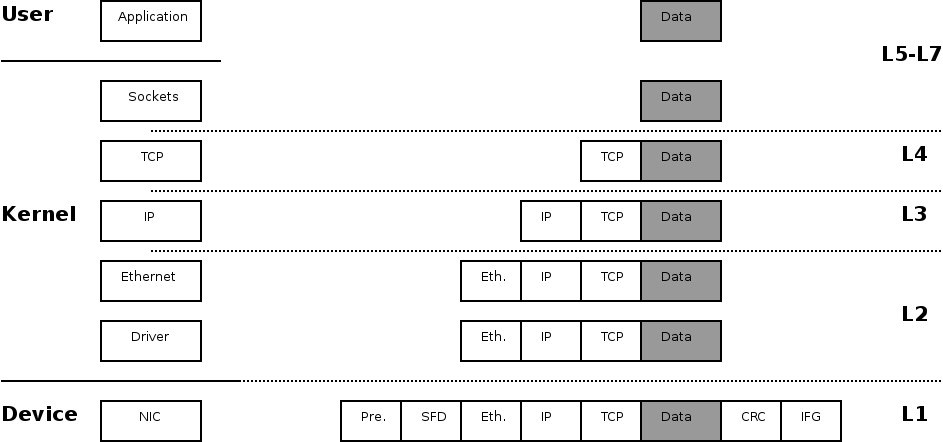
\includegraphics[width=14cm,keepaspectratio]{fig/layers.png}
	\caption{Linux kernel layers}
	\label{fig:linux-layers}
	\bigskip
\end{figure}

Every received incoming frame is passed to the kernel.
On a DMA-capable network card, the kernel allocates a buffer from its memory and passes its descriptor to the
device driver during the device initialisation~\cite{tcpip-in-linux}.
These descriptors are used to store the frames received on the network card by using DMA transfers.
%The device driver instructs the device to use DMA transfers.
A buffer descriptor indicates where the buffer resides in the kernel memory and how big the buffer is~\cite{tcpip-in-linux}.
The purpose of the DMA transfer is to move data without CPU intervention.
Once a complete frame is transferred using a device DMA transfer,
the device raises an interrupt to inform the kernel about the received data~\cite{tcpip-in-linux}.

Each received packet is then handled by a matching L3 protocol handler.
An IPv4 packet is handled by the {\it{ip\_rcv()}} function
and an IPv6 packet by {\it{ipv6\_rcv()}}~\cite{linux-kernel-networking}.
Similarly, each outgoing packet is passed downwards through the layers of the network stack.
The device driver is associated with a specific link type (e.g. Ethernet),
so it knows how to interpret the L2 header
and extract the information about which L3 protocol is encapsulated~\cite{understanding-internals}.

\begin{figure}[H]
	\bigskip
	\centering
	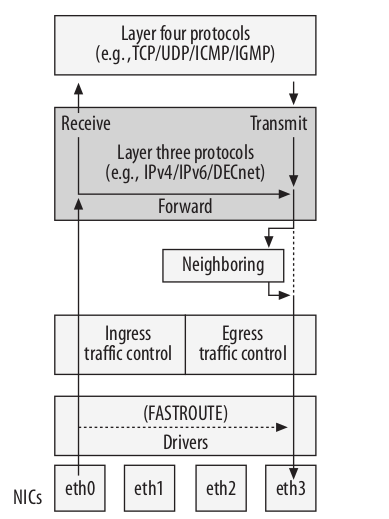
\includegraphics[width=6cm,keepaspectratio]{fig/flow.png}
	\caption{Linux kernel traffic flow (source:~\cite{linux-kernel-networking})}
	\label{fig:linux-flow}
	\bigskip
\end{figure}

Figure~\ref{fig:linux-flow} shows an overview of the traffic flow in the Linux kernel described above.
Parts that are discussed in this thesis include the Forward path for IPv4 packets (routing),
Ingress traffic control, Egress traffic control and the Fastroute feature, which is mentioned briefly
as it is no longer supported~\cite{linux-kernel-networking}.
The hardware of NICs, Neighboring and L4 protocols are not discussed in this thesis.
As the packet passes through different layers of the stack,
the kernel manipulates it using an internal data structure, called {\it{socket buffer}}.
This structure contains the actual packet, but it is not copied between layers.
Instead, a pointer to the structure is passed when passing the packet through the stack~\cite{understanding-internals}.

%=========================================================================
% (c) 2014, 2015 Josef Lusticky

\section{Socket buffer}
The socket buffer ({\it{struct sk\_buff}}, often abbreviated as {\it{skb}}) is an internal kernel data structure that
represents an incoming or outgoing packet.
The socket buffer {\it{struct sk\_buff}} is defined in {\it{include/linux/skbuff.h}} of the kernel source code~\cite{kernel-source}.
A single packet is always stored in its own {\it{skb}}
as the packet crosses through the kernel layers.
Some members of the {\it{skb}} are set sooner or later depending on the direction of the packet~\cite{linux-kernel-networking}.
Listing~\ref{lst:linux-skb} shows a part of the {\it{struct sk\_buff}} definition.
\bigskip
\bigskip
\begin{lstlisting}[caption={Notable members of struct sk\_buff},label={lst:linux-skb}]
struct sk_buff {
  . . .
  struct sock *sk;
  struct net_device *dev;
  . . .
  __be16 protocol;
  unsigned long _skb_refdst;
  . . .
  sk_buff_data_t tail;
  sk_buff_data_t end;
  unsigned char *head,
                *data;

  sk_buff_data_t transport_header;
  sk_buff_data_t network_header;
  sk_buff_data_t mac_header;
  . . .
};
\end{lstlisting}
\bigskip
Every transmitted {\it{skb}} has an associated socket object {\it{*sk}},
which points to the socket that the packet comes from.
It is a network layer representation of sockets.
If the packet is forwarded, then {\it{sk}} is set to NULL,
because it was not generated on the local host~\cite{linux-kernel-networking}.
For incoming packets, the {\it{*dev}} member of skb structure points to the incoming network device,
and for outgoing packets to the outgoing network device~\cite{linux-kernel-networking}.

The {\it{protocol}} member of {\it{skb}} represents the Type or Length field found in the Ethernet header.
If the value is less than 0x0600 then the frame is interpreted as an Ethernet II frame and the field represents Type
(e.g. 0x0800 in case of IP or 0x86DD in case of IPv6).
Otherwise it is interpreted as an 802.3 frame and the field represents Length.
The {\it{\_\_be16}} data type denotes a 2-byte Big Endian value~\cite{kernel-source}.

The {\it{\_skb\_refdst}} member is not assigned immediately upon frame reception,
but it is assigned by a higher-layer protocol handler (e.g. in the IPv4 stack).
The {\it{\_skb\_refdst}} member is used to store a reference to the result of a routing decision,
called destination entry object.
This object is created by the routing subsystem
and it points to the next packet processing function~\cite{linux-kernel-networking}.

The {\it{head}} and {\it{end}} point to the beginning and end of the space allocated to the buffer,
whereas the {\it{data}} and {\it{tail}} are set while moving through the stack according to the layer
which currently processes the packet~\cite{understanding-internals}.
The {\it{sk\_buff\_data\_t}} data type is a typedef to either {\it{char*}} or {\it{unsigned int}}.
In the first case it is a direct pointer to the data, in the later case it represents offset~\cite{kernel-source}.

The {\it{mac\_header}} member is a link layer encapsulation and points to the start of the L2 header in the frame.
Similarly there are {\it{network\_header}} and {\it{transport\_header}} members of {\it{struct sk\_buff}}.

Figure~\ref{fig:linux-skb} shows the discussed members of the {\it{struct sk\_buff}} and their relationship to the Ethernet
frame carrying a TCP/IP packet.

\begin{figure}[H]
	\centering
	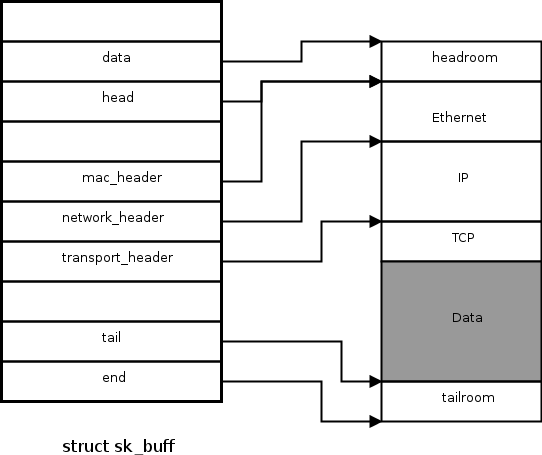
\includegraphics[width=9cm,keepaspectratio]{fig/skb.png}
	\caption{Socket buffer structure}
	\label{fig:linux-skb}
	\bigskip
\end{figure}

According to the {\it{protocol}} member, a pointer to the {\it{skb}}
of the received packet is passed to a higher-layer protocol handler.
In case of an IPv4 packet, it is the {\it{ip\_rcv()}} function,
which is part of the Linux IPv4 stack.


%=========================================================================
% (c) 2014, 2015 Josef Lusticky

\section{IP stack}\label{sec:linux-ip}
The Linux IPv4 stack, or simply the IP stack, claims to be the most RFC-compliant network stack available~\cite{linux-foundation-toe}.
The functions found in the IPv4 stack are responsible for handling IPv4 packets only.
IPv6 packets are handled by the IPv6 stack, which is different,
however, most of the principles of IPv4 processing, apply to IPv6 processing as well~\cite{linux-kernel-networking}.

Figure~\ref{fig:linux-ingress-packet} shows the core functions of the IP stack for ingress packet processing in the Linux kernel.
For the sake of simplicity, the figure shows no IPsec, Fragmentation or IP-Options processing.
The NF\_IP\_* items represent places where the Netfilter hooks can be applied.
Netfilter is an internal kernel framework for packet filtering,
network address translation, port translation, and more~\cite{netfilter}.
Netfilter can be manipulated from user-space using the iptables utility.

\begin{figure}
	\centering
	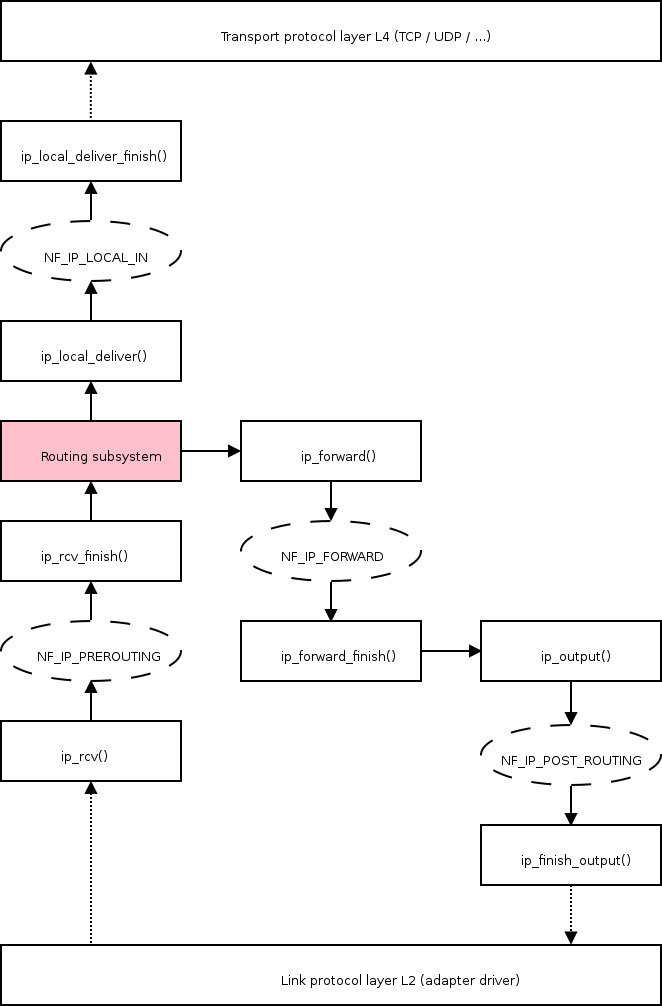
\includegraphics[width=12cm,keepaspectratio]{fig/kernel-layer3-flow.png}
	\caption{Ingress packet processing in the IPv4 stack}
	\label{fig:linux-ingress-packet}
	\bigskip
\end{figure}

The {\it{ip\_rcv()}} function performs mostly sanity checks -
IP version, IP checksum and header length are checked~\cite{kernel-source}.
If the received packet passes all the checks, it proceeds to the NF\_INET\_PRE\_ROUTING hook callback,
if such callback is registered.
If it was not discarded by the netfilter hook,
the {\it{skb}} associtated with the packet is passed to the {\it{ip\_rcv\_finish()}} function,
where a lookup in the routing subsystem is performed.
The routing subsystem mainly assigns the {\it{skb$\rightarrow$\_skb\_refdst}} and it is further discussed in section~\ref{sec:linux-routing}.

Depending on the routing decision, the packet is either dropped with no further processing
or passed to the {\it{ip\_local\_deliver()}} function in case
the local host is the destination, or to the {\it{ip\_forward()}} function in case it needs to be forwarded~\cite{linux-kernel-networking}.
Packets to be delivered on the local host are passed to a higher-layer protocol handler (e.g. TCP)
for further processing.

Packets that are going to be forwarded are passed to the {\it{ip\_forward()}} function.
This function checks and decrements the value of the Time To Live (ttl) field in the IPv4 header.
If it reaches 0, the packet is discarded and an ICMPv4 message with "TTL Count Exceeded" code is sent back~\cite{linux-kernel-networking}.
Moreover, each time a packet is being
forwarded and the TTL is decremented by 1,
the checksum of the IPv4 header must be recalculated,
as its value depends on the IPv4 header, and the TTL is one of the IPv4 header members.
These tasks are done by the {\it{ip\_forward()}} function~\cite{linux-kernel-networking}.
The output processing function for the {\it{skb}} is further set to {\it{ip\_output()}}.
The packet is then passed to the {\it{ip\_forward\_finish()}} function,
which updates forwarding statistics and invokes the output processing function~\cite{linux-kernel-networking}.

The {\it{ip\_output()}} function updates transmission statistics and
assigns the output device to the {\it{skb$\rightarrow$dev}} member.
The packet is then passed to the {\it{ip\_finish\_output()}} function,
which must fragment the packet in case it is larger than the MTU of the {\it{skb$\rightarrow$dev}} device.
The function further takes care of neighboring using Address Resolution Protocol (ARP)~\cite{kernel-source}.
The neighboring subsystem is outside the scope of this thesis,
but in case the link-layer address of the destination is not known,
the packet transmission can be significantly delayed.


%=========================================================================
% (c) 2014, 2015 Josef Lusticky

\section{Routing subsystem}\label{sec:linux-routing}
Routing takes place on L3, so it is entirely kernel's responsibility to forward packets to their destination.
For each packet, incoming or outgoing, a lookup in the routing subsystem is performed~\cite{linux-kernel-networking}.
The decision about whether a packet should be forwarded and which interface it should be sent on is done based on the result of
the lookup in the routing subsystem.
The routing subsystem is a component of the kernel's IP stack and is responsible for forwarding packets and maintaining
the forwarding information base (FIB)~\cite{linux-kernel-networking}.

Familiar routing daemons, such as Quagga or Bird, are entirely user-space applications.
They are not responsible for routing any packet.
Instead, these routing daemons manipulate the kernel's FIB to
contain the selected routes based on
the routing protocol and algorithm they use (OSPF link-state, BGP best path, etc.).
To use these protocols and algorithms,
these user-space daemons usually maintain routing tables of their own, which should not be confused with the
FIB used by the kernel~\cite{linux-kernel-networking}.
The kernel's FIB is manipulated from user-space
either by {\it{ioctl()}} or by modern {\it{Netlink sockets}}~\cite{networking-subsystem-configuration-interface}.

Advanced routing topics, such as multipath and multicast routing are not covered in this thesis.
Multipath routing provides ability to add more than one nexthop to a route~\cite{linux-kernel-networking}.
Otherwise only one nexthop can be specified for a destination.
Multicast routing provides ability to route packets destined to multicast addresses~\cite{linux-kernel-networking}.

The Linux kernel supports up to 255 routing tables that can be used for policy routing.
%The compile-time configuration option {\it{CONFIG\_IP\_MULTIPLE\_TABLES}} enables support for multiple routing tables.
However, the use of multiple routing tables can make a router very complex and therefore
policy routing is beyond the scope of this thesis.
With no policy routing, there are two routing tables created by the kernel while booting - the {\it{local}} FIB table
and the {\it{main}} FIB table.
The {\it{local}} table contains routing entries of local addresses.
Routing entries can be added to the local table only by the kernel.
Adding routing entries to the {\it{main}} table is done by a system
administrator or by routing daemons or as a result of an ICMP Redirect message~\cite{linux-kernel-networking}.

The routing entries of the kernel's FIB table are organised as a Trie structure.
The routing lookup in the Linux kernel uses longest matching prefix lookup algorithm
called FIB TRIE (also known as LC-trie), which performs good for large routing tables.
The routing lookup can consume much of CPU time, depending on the size of the FIB table.
It can also consume much of the memory as the algorithm is rather complex~\cite{linux-kernel-networking}.

A lookup is done by the {\it{fib\_lookup()}} function, defined in the {\it{include/net/ip\_fib.h}} file
of the kernel source code~\cite{kernel-source}.
When the {\it{fib\_lookup()}} function finds a proper entry in the FIB table,
it builds a {\it{fib\_result}} object, which consists of various routing parameters,
including the next hop associated with the outgoing interface~\cite{linux-kernel-networking}.
Listing~\ref{lst:linux-fib-lookup} shows implementation of {\it{fib\_lookup}} when
multiple routing tables configuration is disabled.
%compile-time option CONFIG\_IP\_MULTIPLE\_TABLES is disabled.

\bigskip
\begin{lstlisting}[caption={Implementation of the fib\_lookup() function},label={lst:linux-fib-lookup}]
int fib_lookup(struct net *net, const struct flowi4 *flp, struct fib_result *res)
{
  struct fib_table *table;

  table = fib_get_table(net, RT_TABLE_LOCAL);
  if (!fib_table_lookup(table, flp, res, FIB_LOOKUP_NOREF))
    return 0;

  table = fib_get_table(net, RT_TABLE_MAIN);
  if (!fib_table_lookup(table, flp, res, FIB_LOOKUP_NOREF))
    return 0;

  return -ENETUNREACH;
}
\end{lstlisting}

The {\it{flowi4}} object consists of fields that are important to the IPv4 routing lookup process, including the
destination address, source address, Type of Service (TOS), and more~\cite{linux-kernel-networking}.
In fact the {\it{flowi4}} object defines the key to the lookup in the routing tables.
For IPv6 there is a parallel object named {\it{flowi6}}.
Both are defined in the {\it{include/net/flow.h}} file of the kernel source code~\cite{kernel-source}.
The {\it{fib\_lookup()}} function first searches the {\it{local}} FIB table.
If the lookup fails, it performs a lookup in the {\it{main}} FIB table~\cite{linux-kernel-networking}.
If that fails as well, an error code representing network unreachable is returned.

After a lookup is successfully done, a destination entry
object is built and associated with the {\it{skb}}~\cite{linux-kernel-networking}.
The destination entry object is implemented by {\it{struct dst\_entry}}, defined in the {\it{include/net/dst.h}} file of
the kernel source code~\cite{kernel-source}.
The result of the lookup is referenced by the {\it{struct fib\_result *res}} pointer,
which indirectly references the created {\it{dst\_entry}} object.

The most important members of the {\it{dst\_entry}} structure are two callbacks named {\it{input}} and {\it{output}}.
These callbacks are assigned to be proper handlers according to the routing lookup result.
For incoming unicast packets destined to the local host, the {\it{input}} callback is set to
{\it{ip\_local\_deliver()}}, and for incoming packets that should be forwarded,
this input callback is set to {\it{ip\_forward()}}.
For a packet generated on the local machine and sent away,
the output callback is set to {\it{ip\_output()}}~\cite{linux-kernel-networking}.
Listing~\ref{lst:linux-dst} shows a part of the {\it{struct dst\_entry}} definition.
\bigskip
\begin{lstlisting}[caption={Destination callback members of struct dst\_entry},label={lst:linux-dst}]
struct dst_entry {
  . . .
  int (*input)(struct sk_buff *);
  int (*output)(struct sk_buff *);
  . . .
}
\end{lstlisting}

A reference to the {\it{dst\_entry}}, which was created as a result of the routing decision,
is assigned to the {\it{skb$\rightarrow$\_skb\_refdst}} member.
The {\it{ip\_rcv\_finish()}} function further calls the {\it{input}} callback
which passes the {\it{skb}} either to the local host processing or to forwarding, as described in section~\ref{sec:linux-ip}.
In case of forwarding, the {\it{output}} callback is further set to the {\it{ip\_output}} function by the
{\it{ip\_forward\_finish()}}, as described in section~\ref{sec:linux-ip},

In terms of performance, there is currently not much space for improvements as
each {\it{skb}} must be handled separately and must be passed to the described functions of the IP stack.
In kernels prior to 3.6, there was an IPv4 routing cache with a garbage collector~\cite{linux-kernel-networking}.
The IPv4 routing cache was removed in kernel 3.6 (released in July 2012),
as it proven to be inefficient and vulnerable to DoS attacks~\cite{linux-cache-removing}.

There used to be a feature called Fastroute that allowed device drivers to route incoming traffic during
interrupt context using a small cache.
The packets were forwarded to the outgoing interface
without having to pass through the higher layer (IP)~\cite{linux-kernel-networking}.
However, this feature is not compatible with other important features, such as Netfilter firewall or advanced routing,
for the simple reason that this low-level forwarding would bypass them.
Starting with the 2.6.8 kernel, Fastroute is no longer supported and
its implementation was removed from the Linux kernel~\cite{linux-kernel-networking}.

As discussed above, the L3 packet processing and routing handle packets associated with their own {\it{skb}}.
However, the lower-layer part of the networking code can provide significant improvements
before the {\it{skb}} enters the {\it{ip\_rcv()}} function.
The improvements depend on how this code handles the ingress frames.


%=========================================================================
% (c) 2014, 2015 Josef Lusticky

\section{Ingress traffic processing}\label{sec:linux-ingress}
The traditional way of processing frames from NIC is interrupt-driven~\cite{linux-kernel-networking}.
Each incoming frame is an asynchronous event which raises a hardware interrupt.
Interrupt handlers run asynchronously with either the current interrupt level disabled or with all
interrupts disabled~\cite{lkd2}.
The handlers could interrupt other potentially important code, therefore they need to run as quickly as possible.
Interrupt handlers immediately respond to hardware and perform time-critical actions,
however, other less critical work should be deferred to a later point when interrupts are enabled~\cite{lkd2}.

Upon frame reception, the hardware interrupt handler of the network adpater
performs the following immediate tasks:~\cite{understanding-internals}
\begin{enumerate}
\item Copies the frame into an {\it{sk\_buff}} data structure.
If DMA is used by the device, the kernel needs only to initialise a buffer and pass its descriptors to the driver,
which instructs the device to use DMA.
The received frame is then copied by a DMA transfer.
\item Initialises some of the {\it{sk\_buff}} members for later usage by upper network layers,
notably the {\it{protocol}} member, which identifies the higher-layer protocol handler and will play a major role later.
\item Updates some other parameters private to the device, such as variables for statistical purposes.
\item Signals the kernel about the new frame by scheduling the NET\_RX\_SOFTIRQ softirq for execution.
\end{enumerate}

To keep the execution of the handler as short as possible,
further frame processing is performed later in the NET\_RX\_SOFTIRQ routine.
This softirq routine actually performs an interrupt-related work
not performed in the hardware interrupt handler~\cite{understanding-internals}.
The routine further passes the received frame
to the corresponding L3 protocol handler according to the {\it{protocol}} member of the {\it{skb}}~\cite{lkd2}.
In case of IPv4, this is the {\it{ip\_rcv()}} function described in section~\ref{sec:linux-routing}.
Moreover, the softirq routine is threaded and can run concurrently on different CPUs~\cite{lkd2}.

However, such method of packet processing became insufficient with the emerge of high-speed network cards.
Even a moderately busy interface can handle thousands of packets per second
and per-packet interrupts quickly overwhelm the processor with interrupt-handling work~\cite{low-latency-ethernet-device-polling}.
On the way towards high-speed packet processing on the host CPU,
packet processing in the network stack must have been adapted.

NAPI ("New API", though not so new anymore)
is an interrupt mitigation mechanism used with network devices~\cite{reworking-napi}.
NAPI mixes interrupts with polling and gives higher performance under high traffic load
than the old approach, by reducing significantly the load on the CPU~\cite{understanding-internals}.

%=========================================================================
% (c) 2014, 2015 Josef Lusticky

\subsection{NAPI}\label{subsec:linux-ingress-napi}
NAPI was first introduced during the Linux kernel 2.5 development cycle as
an extension to the device driver packet processing framework,
which is designed to improve the performance of high-speed networking~\cite{linux-foundation-napi}.

A NAPI-compliant device driver must implement a {\it{poll()}} function used by the kernel to fetch the received frames.
The first frame received causes a hardware interrupt and its handler to run as usual.
In the handler, however, the driver disables interrupts from the device
and calls the {\it{netif\_rx\_schedule()}} function.
This function adds the device to the kernel's {\it{poll\_list}} and schedules the NET\_RX\_SOFTIRQ routine.
From now on, the task of delivering more incoming frames from
the device's queue is delegated to the kernel~\cite{understanding-internals}.

In the NET\_RX\_SOFTIRQ routine, the kernel iterates over the polll\_list and keeps calling
the {\it{poll()}} function of the device driver to fetch the frames from the device's ingress queue (implemented as a ring buffer).
The kernel fetches the packets and passes them to the higher-layer protocol handler for further processing~\cite{linux-kernel-networking}.
The {\it{poll()}} function is called with a maximum number
of packets ({\it{budget}}) it is allowed to feed into the kernel.
It should process up to that many packets and return~\cite{reworking-napi}.
Figure~\ref{fig:linux-napi-workflow} shows the NAPI workflow described above.

\begin{figure}
	\centering
	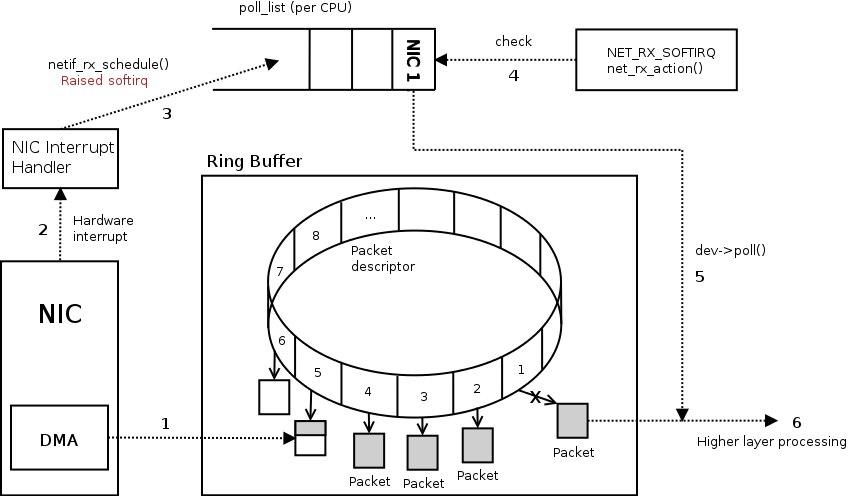
\includegraphics[width=15cm,keepaspectratio]{fig/napi-workflow.png}
	\caption{NAPI workflow}
	\label{fig:linux-napi-workflow}
\end{figure}

When the kernel is ready to deal with more packets, the {\it{poll()}} function of the next device
in the {\it{poll\_list}} will be called.
The scheduled devices are probed in a round-robin manner.
The total number of packets fetched from devices in the {\it{poll\_list}} is limited.
If it was not sufficient to serve all devices in the {\it{poll\_list}} and the kernel should release the CPU,
the devices have to wait for the next NET\_RX\_SOFTIRQ run~\cite{understanding-internals}.
The softirq NET\_RX\_SOFTIRQ processing for NAPI-compliant drivers
is implement by the {\it{net\_rx\_action()}} function defined in {\it{net/core/dev.c}}~\cite{kernel-source}.
The function overview is shown in figure~\ref{fig:linux-softirq-napi}.

\begin{figure}
	\centering
	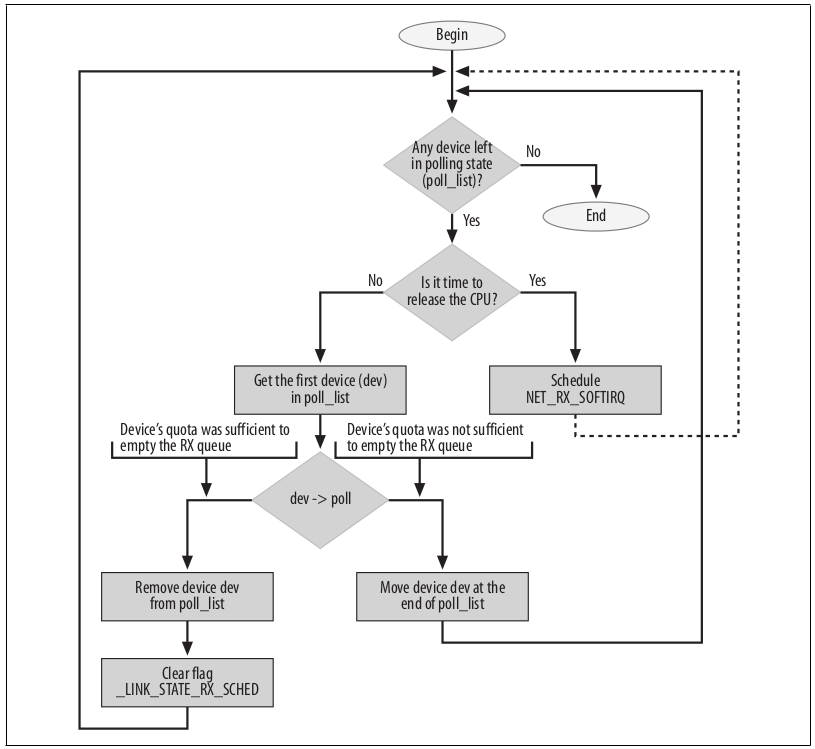
\includegraphics[width=14.5cm,keepaspectratio]{fig/net_rq_softirq.png}
	\caption{Softirq NAPI routine {\it{net\_rx\_action}} (source:~\cite{understanding-internals})}
	\label{fig:linux-softirq-napi}
\end{figure}

When a device driver uses NAPI, it is up to
the driver to implement any congestion control mechanism.
This is because ingress frames are kept in the NIC's memory or in the receive ring buffer managed by the driver,
and the kernel cannot keep track of traffic congestion~\cite{understanding-internals}.
When the host becomes congested, the packets are lost because of not enough space in the ring buffer.
The packets that are going to be lost are not fed into the network stack, so they take no CPU time~\cite{haifux-lecture}.

When a device cannot clear out its ingress queue in a single poll,
it has to wait until the next call.
The kernel keeps calling the driver's {\it{poll()}} function until
it empties the device's ingress queue out~\cite{understanding-internals}.
At that point, there is no need anymore for polling.
The device is removed from the {\it{poll\_list}}
and the device driver can re-enable interrupt notifications for the device~\cite{understanding-internals}.
Nowadays, almost every driver supports the NAPI feature~\cite{linux-kernel-networking}.

NAPI reduces interrupt load on the system and lowers the CPU utilisation under heavy load,
but it increases latency as packets are not processed as quickly~\cite{linux-foundation-napi}.
User-space applications that need the lowest
possible latency and are willing to pay a cost of higher CPU utilisation,
can use a capability for busy polling on sockets (called Low Latency Sockets), which was added in kernel 3.11~\cite{linux-kernel-networking}.
Low Latency Sockets eliminate the cost of the interrupt and context switch
and provide latency very close to the hardware latency~\cite{intel-lls}.

In addition to NAPI, various offload engines were designed to take over some responsibilities of the networking code
and implement them in hardware.


%=========================================================================
% (c) 2014, 2015 Josef Lusticky

\subsection{Receive offloads}\label{subsec:linux-ingress-offloads}
Network adapter vendors have been adding protocol support to their cards.
This support can vary from the simple (checksumming of packets, for example)
through to full TCP/IP implementations~\cite{linux-and-tcp-offload-engines}.

To mitigate CPU load spent on TCP overhead completely, the TCP Offload Engine (TOE) is implemented in several NICs.
TOE features a full TCP/IP implementation in adapter, including the TCP connection management.
However, Linux has never supported the TOE features of any network cards~\cite{linux-and-tcp-offload-engines}.
Vendors have made modifications to the Linux kernel to support TOE,
and these changes have been submitted for kernel inclusion but were rejected~\cite{linux-foundation-toe}. 

Linux kernel engineers currently feel that the full network stack offload
that TOE provides has little merit~\cite{linux-foundation-toe}.
TOE shorts out much of the Linux networking code, described in the previous sections.
In the process, it cuts out features like Netfilter, traffic control, and more.
The Linux networking stack is easy to fix when a bug or security issue comes up~\cite{linux-and-tcp-offload-engines}.
If a security problem turns up in a TOE adapter, instead, there is very little which can be done to fix it.
Linux engineers claim that 100~Mbps TOE adapters
(which used to be the bleeding-edge high speed)
are now slower than the Linux networking stack.
So any performance advantage from TOE is a temporary thing, but once the TOE's code is merged, it must be supported.
As a result of this, TOE support might become a long-term maintenance burden~\cite{linux-and-tcp-offload-engines}.

Although inclusion of TOE support was rejected, there are ways to obtain TOE's performance without
necessitating stateful support in the cards~\cite{linux-and-tcp-offload-engines}.
Everything that is worthwhile can be done with stateless offloads.
One of the simplest stateless offload technique is computing checksums in hardware.
With receive (Rx) checksum offload, IP, TCP and UDP checksums are checked in the hardware of the NIC upon frame reception.

While checksum offload provides some performance improvement,
a large portion of per-packet processing overhead remains.
Each packet is passed through the entire IP stack, as described in section~\ref{sec:linux-ip}.
Dealing with each single packet takes a significant amount of the CPU time, particularly on high-speed Ethernet links that
can produce millions of packets per second.

Given the importance of per-packet overhead, it makes sense to raise the MTU.
However, most connections of interest go across the Internet,
and those are all bound by the lowest MTU in the entire path.
As noted in section~\ref{sec:40gbe-compatibility}, the IEEE has determined no support for frames with MTU larger than 1500.
Protocol-based mechanisms for MTU discovery exist, but they do not work well on the Internet,
because in particular, a lot of firewall setups do not allow them to work~\cite{jls2009-gro}.

If the kernel can not use a larger MTU, it can pretend that it is using a larger MTU.
An optimisation technique to pretend larger MTU is provided by the Large Receive Offload (LRO).
LRO merges packets of the same TCP flow together,
creating one large super-frame, before it is passed to the higher network layers~\cite{jls2009-gro}.
Merging multiple packets and processing them as a single packet
reduces CPU overhead and thus improves performance~\cite{linux-kernel-networking}.
The merging can be done either in the driver or in the hardware.
Even LRO emulation in the driver has performance benefits~\cite{jls2009-gro}.

Since LRO merges everything of the same TCP flow into one large super-frame,
the differences in the headers of these packets are lost~\cite{jls2009-gro}.
If a system is acting as a router, it should not be changing the headers on packets as they pass through,
because it brakes the end-to-end principle and can significantly impact performance~\cite{linux-kernel-networking}.

A generic solution was introduced by the Generic Receive Offload (GRO) to mitigate the problems of LRO.
In GRO, the criteria for which packets can be merged is greatly restricted.
The MAC headers must be identical and only a few TCP or IP headers can differ -
checksums are necessarily different and the Identification field is allowed to increment~\cite{jls2009-gro}.
As a result of these restrictions, merged packets can be later resegmented losslessly
and therefore the GRO feature can be used by a system
acting as a router without braking the end-to-end principle~\cite{jls2009-gro}.
However, GRO still requires the L4 protocol to have its own segmentation support
and it is currently restricted to TCP only~\cite{linux-kernel-networking}.

When using GRO, merging packets of the same flow into one large super-frame must be time-limited.
In combination with NAPI, there is no need for any special waiting code -
the kernel already calls the driver's poll method for new packets occasionally and processes them in batches.
Thus, GRO can simply be performed at NAPI poll time without introducing any additional latency~\cite{jls2009-gro}.
The GRO feature improves network performance
and it deprecated LRO in recent kernels~\cite{linux-kernel-networking}.
Figure~\ref{fig:linux-rcv-offloads} shows comparison of ingress frames processing
with and without the above described offload mechanisms.

\begin{figure}
	\centering
	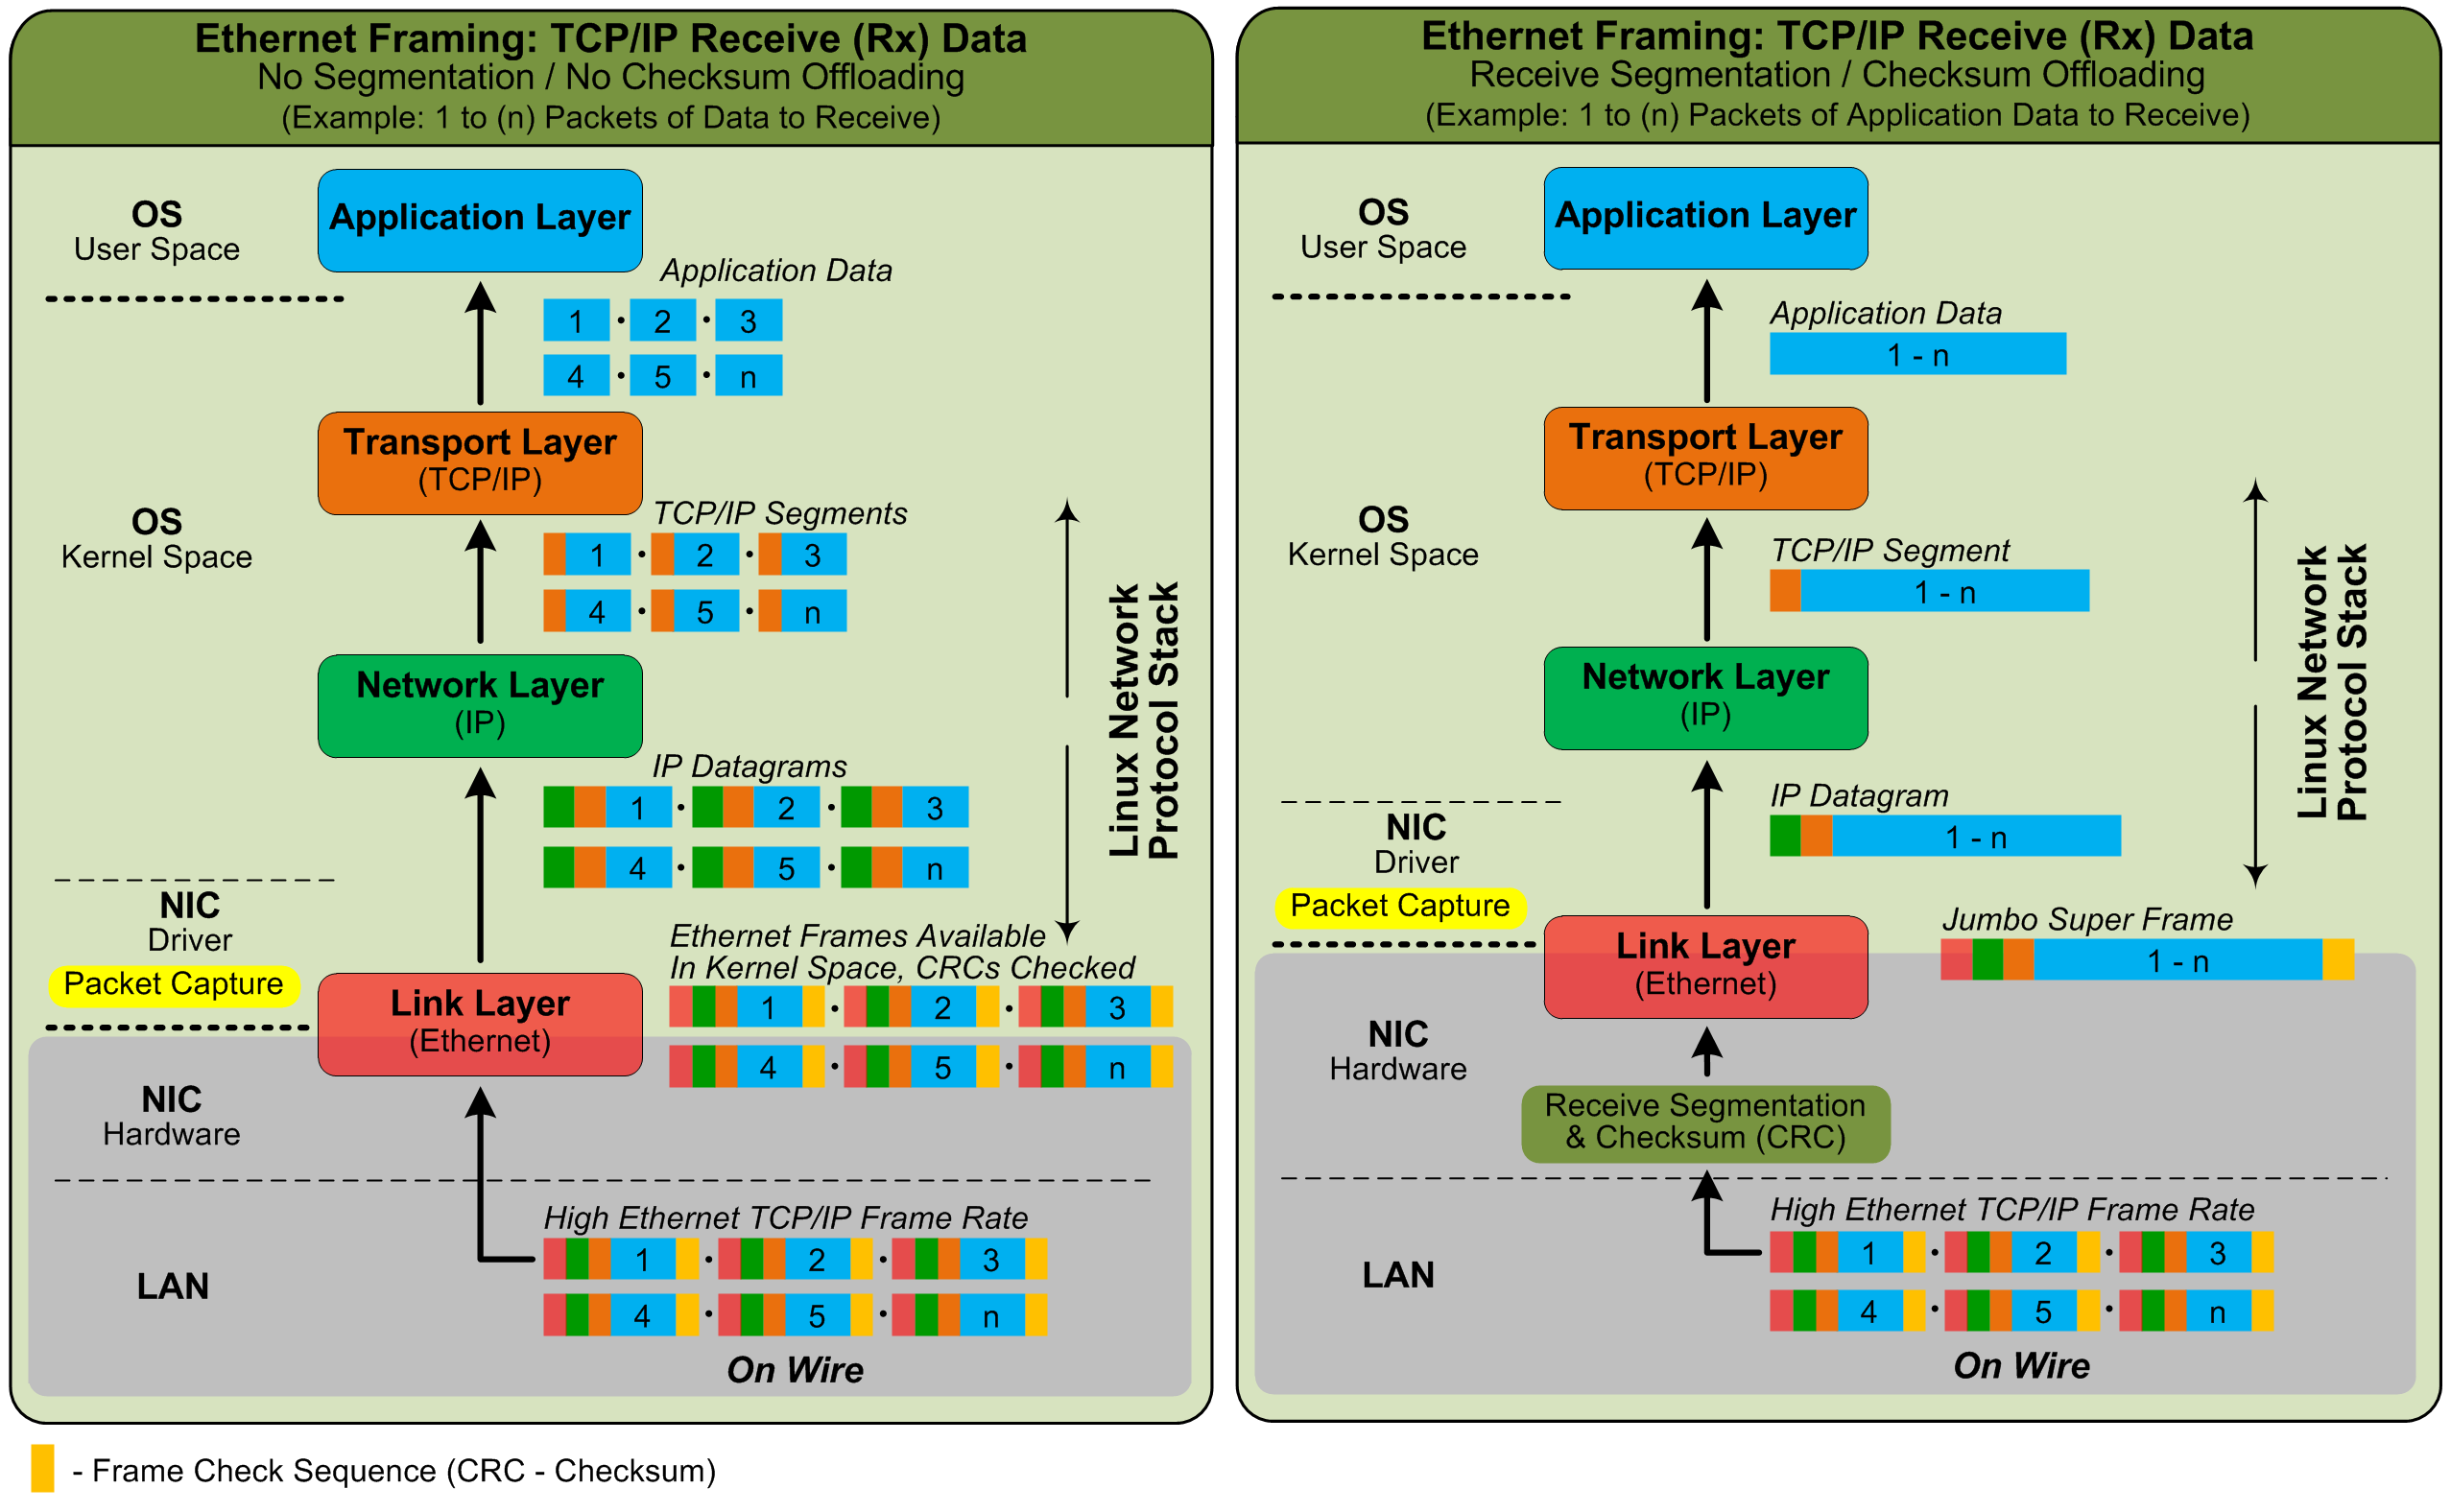
\includegraphics[width=15cm,keepaspectratio]{fig/rcv-offloads.png}
	\caption{Receive offloads (source:~\cite{nst-offloads})}
	\label{fig:linux-rcv-offloads}
	\bigskip
\end{figure}



%=========================================================================
% (c) 2014, 2015 Josef Lusticky

\section{Egress traffic processing}\label{sec:linux-egress}
The previous sections described how the frame reception works and the way they are passed when
the routing subsystem decides to forward them.
After the routing decision is made and the {\it{skb}} is passed to the {\it{ip\_finish\_output()}} function,
it is further passed back to the link layer part of the stack.
This part of the Linux networking also provides interface to the device drivers
and handles traffic control~\cite{understanding-internals}.

In reference to the egress traffic processing, there are two important functions in this part of the stack -
{\it{dev\_queue\_xmit()}} and {\it{dev\_hard\_start\_xmit()}}.
The {\it{ip\_finish\_output()}} function of the IPv4 stack passes the outgoing {\it{skb}}
to the {\it{dev\_queue\_xmit()}} function, which determines whether the device is queueless of queueful~\cite{understanding-internals}.
If the device is queueless, such as Loopback or Virtual interface, then the {\it{skb}} is passed to
{\it{dev\_hard\_start\_xmit()}} directly without any traffic control mechanism involved.
The {\it{dev\_hard\_start\_xmit()}} function further prepares the {\it{skb}} for transmission
and passes it to the transmission function of the device driver,
which instructs the device to transmit the frame on the wire~\cite{understanding-internals}.

If the device is queueful, such as almost any hardware network adapter, {\it{dev\_queue\_xmit()}}
executes the traffic control first~\cite{understanding-internals}.
The traffic control implemented in the Linux kernel uses algorithms known as queuing disciplines
(often abbreviated as qdisc)
to arrange the frames in the most efficient order for transmission~\cite{understanding-internals}.
Figure~\ref{fig:linux-egress-packet} shows the above described part of the stack.
\begin{figure}
	\centering
	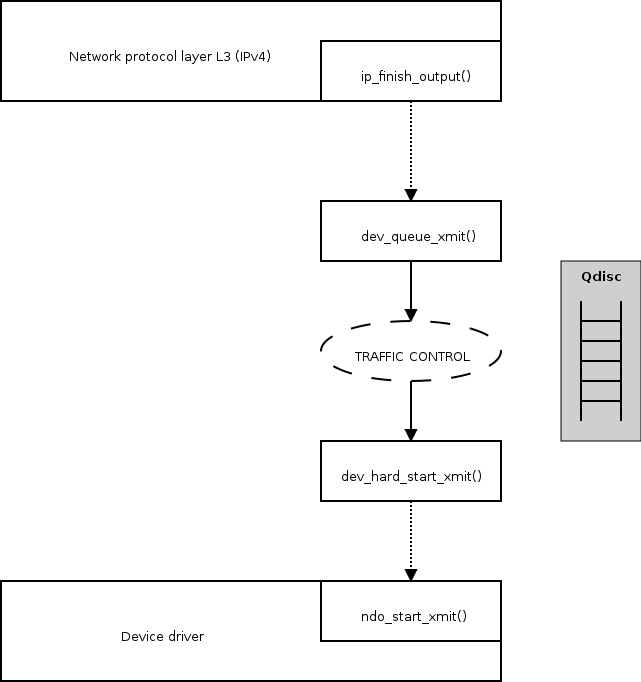
\includegraphics[width=10cm,keepaspectratio]{fig/kernel-layer2-flow.png}
	\caption{Egress packet processing}
	\label{fig:linux-egress-packet}
	\bigskip
\end{figure}

The default queuing discipline for every network device where
no custom configuration has been applied is fifo\_fast~\cite{linux-kernel-networking}.
As the name suggests, the fifo\_fast is a classless First In First Out discipline,
that is, the first packet to get in, is going to be the first to be sent~\cite{tcpip-in-linux}.

After the packet has been selected for transmission by the traffic control, it is passed to the
{\it{ndo\_start\_xmit()}} function, which is implemented by the device driver~\cite{kernel-source}.
The packet is inserted to the hardware transmit queue by the driver.

Linux kernel supports multiple queuing disciplines, that can be configured by the {\it{tc}} utility.
A more detailed discussion of the traffic control and its queuing disciplines is outside the scope of this thesis.
Currently two qdiscs are optimised for multiqueue devices.
The first is the default pfifo\_fast qdisc.
This qdisc supports one qdisc per hardware queue.
The mq (multiqueue) qdisc is a dummy scheduler.
It is used by default for multiqueue devices instead of the regular pfifo\_fast qdisc,
but can also be attached manually to restore multiqueue behaviour
after attaching a non-multiqueue (shared) qdisc~\cite{kernel-doc-multiqueue}.

%%%

The networking subsystem has been assigned two different softirqs -
NET\_RX\_SOFTIRQ handles incoming traffic and NET\_TX\_SOFTIRQ handles outgoing traffic.
Because different instances of the same softirq handler can run concurrently on different CPUs,
networking code is both low latency and scalable~\cite{understanding-internals}.

\subsection{Transmit offloads}
Most of the adapters that support receive checksum offload,
also support its counter-part option to offload transmission (Tx) checksums.
Tx checksum offload calculates TCP/UDP and
IP checksums of the packets in the hardware before they are transmitted on the wire.

%TODO Scatter-gather feature allows the network adapter to read from and write to
%non-contiguous areas during direct memory access (DMA)~\cite{linux-kernel-networking}.

A counter-part of LRO is TCP Segmentation Offload (TSO).
With a TSO-capable adapter, the kernel can prepare much larger packets (e.g. 64KB)
for outgoing data and the adapter will re-segment the data into smaller packets according to the MTU~\cite{jls2009-gro}.
TSO is well supported in Linux -
for systems which are engaged mainly in sending of data, it is sufficient to make 10Gb line-rate at full speed~\cite{jls2009-gro}.
TSO reduces the necessary CPU load, bus overhead, and cache impact to send a series of packets,
but it still does not require the adapter to actually know
anything about specific TCP connections -
the kernel still has to deal with the TCP states and ACKs~\cite{linux-and-tcp-offload-engines}.

The TCP Segmentation Offload is designed to work with TCP exclusively.
To mitigate this issue, the Generic Segmentation Offload (GSO) was implemented, which is not limited to TCP.
Performance improves even if the feature is emulated in the driver~\cite{jls2009-gro}.
Figure~\ref{fig:linux-tx-offloads} shows comparision of egress processing
with and without the above described offload mechanisms.
\begin{figure}
	\centering
	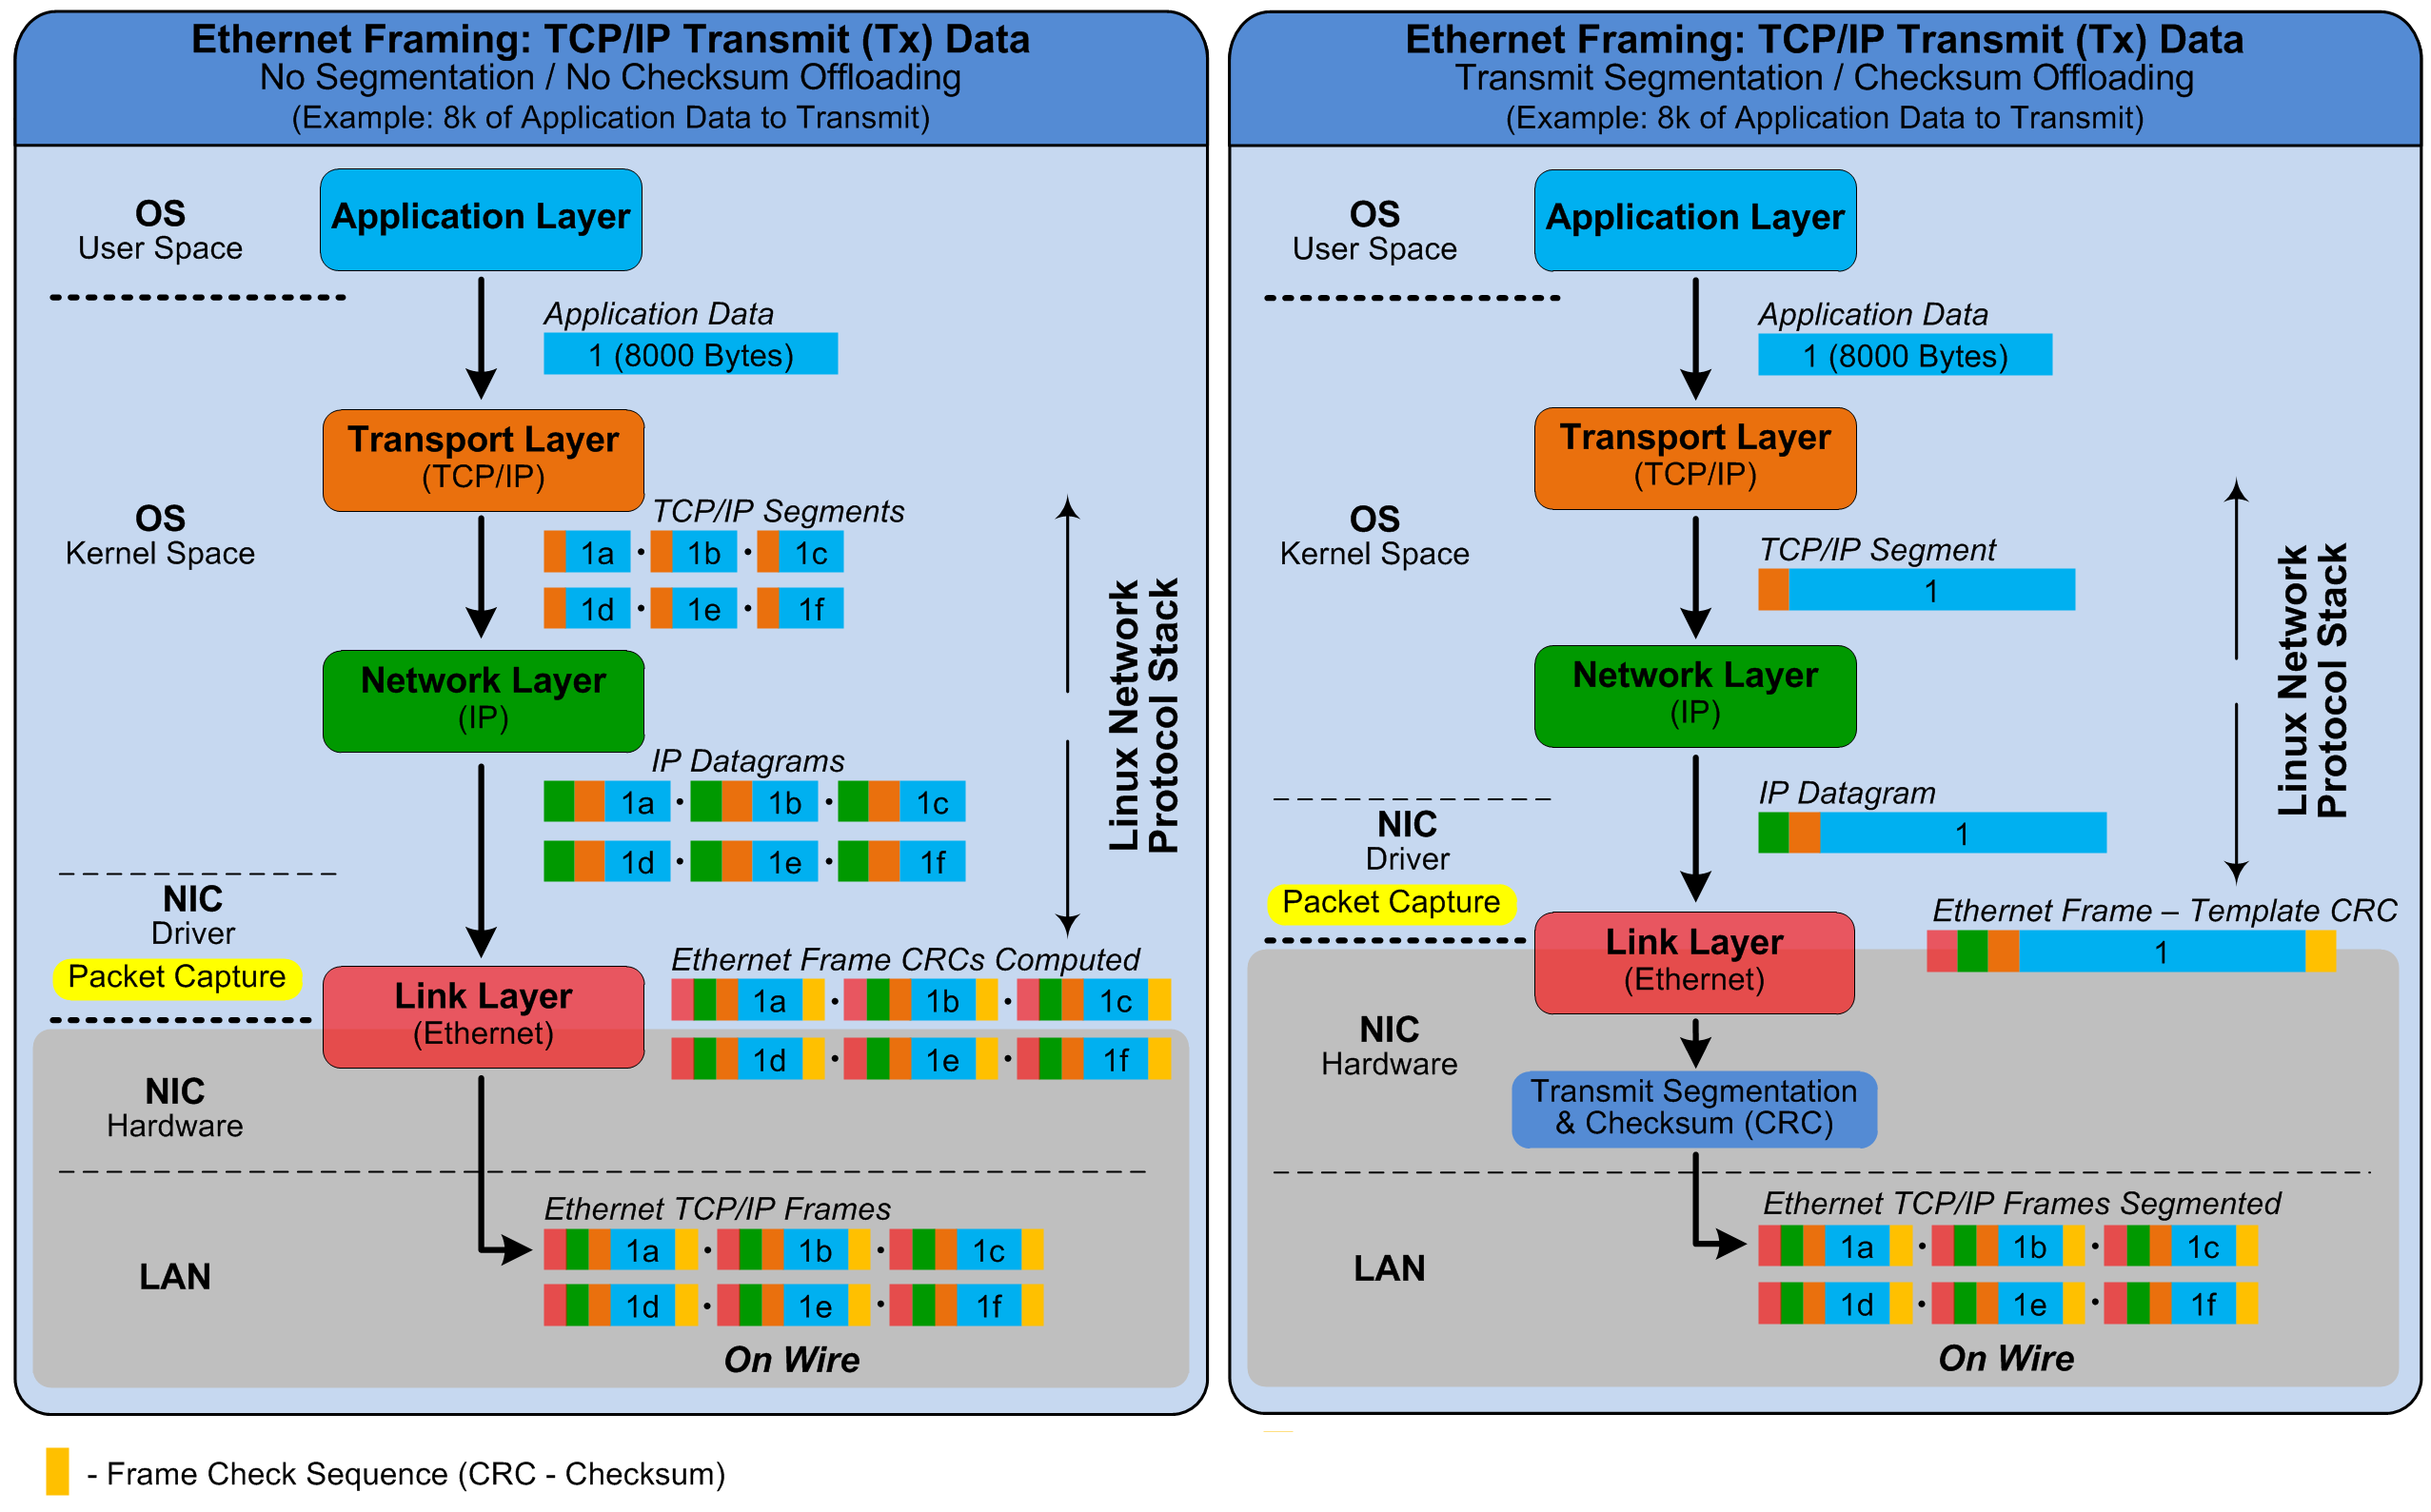
\includegraphics[width=15cm,keepaspectratio]{fig/tx-offloads.png}
	\caption{Transmit offloads (source:~\cite{nst-offloads})}
	\label{fig:linux-tx-offloads}
	\bigskip
\end{figure}

%Large Receive Offload (LRO) packets are dropped in forwarding.
%Forwarding a large SKB, which was
%built by LRO, is not acceptable because it will be larger than the outgoing MTU.
%Therefore, when LRO is enabled the
%SKB is freed and the method returns NET\_RX\_DROP.
%Generic Receive Offload (GRO) design included forwarding
%ability, but LRO did not~\cite{linux-kernel-networking}.


%=========================================================================
% (c) 2014, 2015 Josef Lusticky

\section{Multiqueue adapters and scaling}\label{sec:linux-scaling}
One of the fundamental data structures in the networking subsystem is the transmit queue associated with each device.
As described in section~\ref{sec:linux-egress}, the core networking code will call the driver's {\it{ndo\_start\_xmit()}}
function to let the driver know that a packet is ready for transmission~\cite{mq-networking}.
The driver feeds that packet into hardware's transmit queue,
which results in a data structure which is shown in figure~\ref{fig:linux-queue-old}.
\begin{figure}
	\centering
	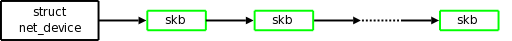
\includegraphics[width=11cm,keepaspectratio]{fig/net-queue-old.png}
	\caption{Single queue device (source:~\cite{mq-networking})}
	\label{fig:linux-queue-old}
\end{figure}

This scheme has worked well for years, but it does not map well to devices which have multiple transmit queues.
The multiqueue devices need each transmit queue to be scheduled independently.
10 and 40~Gigabit Ethernet devices with multiple transmit queues are very common~\cite{mq-networking}.

To provide an independent scheduling of a transmit queue,
a new {\it{netdev\_queue}} structure is implemented in the Linux kernel.
The {\it{netdev\_queue}} structure encapsulates all of the information about a single transmit queue,
and it is protected by its own lock.
Multiqueue device drivers set up an array of these structures according to the number of queues.
The {\it{mq}} (multiqueue) queueing  discipline uses the array to attach a specific {\it{qdisc}} to each queue.
The {\it{mq}} discipline is a dummy scheduler, which is used by default
for multiqueue devices instead of the regular {\it{pfifo\_fast}} discipline~\cite{kernel-doc-multiqueue}.
Figure~\ref{fig:linux-queue-mq} shows the new data structure.
\begin{figure}
	\centering
	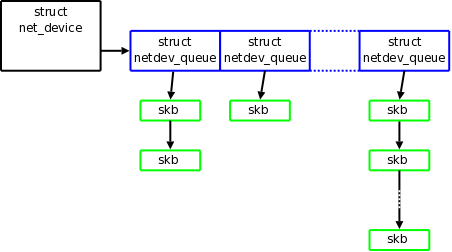
\includegraphics[width=11cm,keepaspectratio]{fig/net-queue-mq.png}
	\caption{Multiqueue device (source:~\cite{mq-networking})}
	\label{fig:linux-queue-mq}
\end{figure}

In addition to multiple transmit queues,
modern high-speed network adapters support multiple receive queues as well~\cite{mellanox-product-brief}.
The principle described above also applies to the receive queues in the Linux kernel.
The multiqueue support allows to scale the network load in multiprocessor systems.
Such scaling is provided by processing each queue by a different CPU~\cite{kernel-doc-scaling}.
The NIC distributes packets to the queues by applying a filter that assigns each packet to one of the receive queues.
The filter is a hash function (usually Toeplitz hash algorithm) over the network and transport layer headers of the packet
and a hash key, which is stored in the NIC's memory.
This mechanism is generally known as Receive Side Scaling (RSS)
and its goal is to increase performance uniformly~\cite{kernel-doc-scaling}.

Network adpaters that do not support RSS but have multiple receive queues can still benefit from multiprocessor scaling
by using Receive Packet Steering (RPS), which is a software implementation of RSS~\cite{kernel-doc-scaling}.
However, there are some disadvantages of RPS against the hardware-based RSS.
The calculation of the hash requires accessing data from the packet header.
That access will necessarily involve one or more cache misses on the CPU running the RPS code -
that data was just put there by the network interface and thus cannot be in any CPU's cache~\cite{receive-packet-steering}.
Once the packet has been passed over to the CPU which will be doing the real work,
that cache miss overhead is likely to be incurred again.
Moreover, the targeted CPU is notified by an inter-processor interrupt,
which introduces another overhead.
If the NIC supports RSS and it is configured to map each hardware
receive queue to a single CPU, then RPS is redundant and unnecessary~\cite{kernel-doc-scaling}.

The network transmission scaling is implemented by the
Transmit Packet Steering in the Linux kernel.
Transmit Packet Steering (XPS) is a mechanism for intelligently selecting
which transmit queue to use when transmitting a packet on a multiqueue device~\cite{kernel-source}.
To accomplish this, there is a configurable mapping from CPU to hardware queues.
The goal of the mapping is usually to assign the queues exclusively to a subset of CPUs, which reduces
contention on the device queue lock since fewer CPUs contend for the same queue.
Contention can be eliminated completely if each CPU has its own transmit queue.
Moreover, the cache miss rate on transmit completion is also reduced since a particular CPU
is serving just a subset of transmit queues~\cite{kernel-doc-scaling}.

Apart from load distribution, the above described mechanism also minimise cache miss rates when configured properly.
The most significant is a cache miss of a hardware interrupt handler for the particular queue,
queue lock cache miss and packet metadata in its {\it{sk\_buff}}.
RPS and RFS were introduced in kernel version 2.6.35
and XPS in 2.6.38~\cite{kernel-doc-scaling}.

To complete the list, there are two additional network scaling mechanisms implemented in the Linux kernel - 
Receive Flow Steering and Accelerated Receive Flow Steering.
Both provide assigning incoming packets to the CPU that the destined user-space application runs on.
The difference between them is that the Accelerated Receive Flow Steering is implemented in the NIC's hardware,
whereas Receive Flow Steering is a software implementation.
Since these two mechanisms provide network scaling to user-space applications, they will not be discussed further in
this thesis~\cite{kernel-doc-scaling}.

